\newpage
\subsection{Diagram of the interior layout}
\begin{figure}[!h]
    \centering
    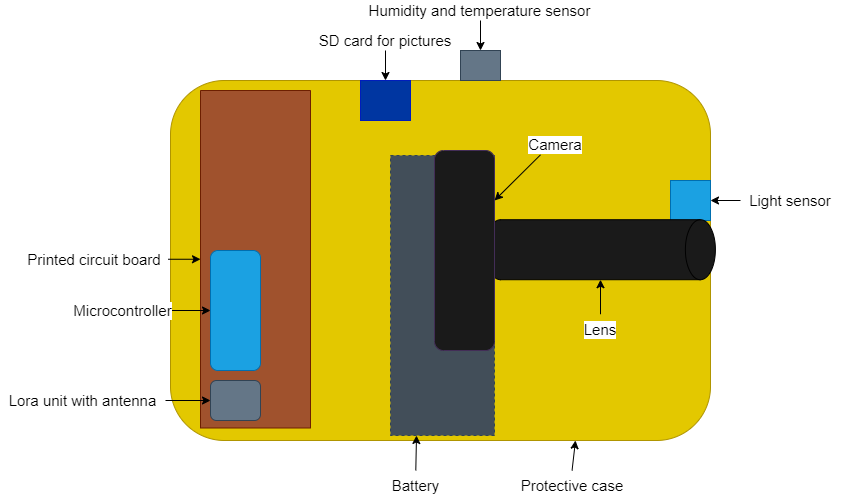
\includegraphics[width=0.9\textwidth]{\currfiledir/figures/interieur_layout.png}
    \caption{Schematic of the system inside the box (upper view)}
\end{figure}

\noindent This diagram shows the arrangement of the components inside the box. These components work together to create a functional unit that can capture and storing images.\\
The microcontroller is the brain of the system, responsible for processing the input data from the sensors and controlling the camera, as well as other functions such as power management and communication.\\
The lens and camera work together to capture high-quality images, which can be stored on the SD card for researcher.\\
The protective case ensures that the system is safe from damage and can withstand harsh environmental conditions.\\
The LoRa unit with its antenna enables the system to communicate wirelessly over long distances, making it ideal for remote monitoring and surveillance applications.\\
The printed circuit board serves as the backbone of the system, connecting all the components together and providing the necessary power and signals for their operation. The motion sensor on the PCB is responsible for detecting any movement of the system and transmitting this information to the base camp where the researchers are located.